\documentclass[preprint,12pt]{elsarticle}

\journal{Fuzzy Sets and Systems}

\usepackage[T1]{fontenc}
\usepackage{lmodern}
\usepackage{amsmath,amssymb,amsthm,mathtools}
\usepackage{booktabs}
\usepackage{tabularx}
\usepackage{array}
\usepackage{enumitem}
\usepackage{xcolor}
\usepackage{graphicx}
\usepackage{tikz}
\graphicspath{{figures/}}
\usepackage[colorlinks,linkcolor=black,citecolor=black,urlcolor=black]{hyperref}
\usepackage{orcidlink}
\usepackage[nameinlink,noabbrev]{cleveref}

\newtheorem{theorem}{Theorem}[section]
\newtheorem{lemma}[theorem]{Lemma}
\newtheorem{proposition}[theorem]{Proposition}
\newtheorem{corollary}[theorem]{Corollary}
\theoremstyle{definition}
\newtheorem{definition}[theorem]{Definition}
\newtheorem{example}[theorem]{Example}
\newtheorem{remark}[theorem]{Remark}
\newtheorem{question}[theorem]{Open question}
\crefname{question}{open question}{open questions}
\Crefname{question}{Open question}{Open questions}
% elsarticle prints the appendix number as ``Appendix A'' already
\crefformat{appendix}{#2#1#3}
\Crefformat{appendix}{#2#1#3}

\newcommand{\R}{\mathbb{R}}
\newcommand{\K}{\mathcal{K}}
\newcommand{\lo}[1]{\underline{#1}}
\newcommand{\up}[1]{\overline{#1}}
\newcommand{\abs}[1]{\lvert #1\rvert}
\newcommand{\eps}{\varepsilon}

% Information that only the authors can supply. Every \fillin must be replaced before submission;
% search for "fillin" to find them all.
\DeclareRobustCommand{\fillin}[1]{\textcolor{red}{\textbf{TO FILL: #1}}}

\biboptions{sort&compress}
\emergencystretch=2em
\setlength{\belowcaptionskip}{6pt}   % captions stand above the tables
\journal{Fuzzy Sets and Systems}

\begin{document}

\begin{frontmatter}

\title{Which Admissible Orders Make Interval Max-Pooling Inclusion-Preserving? A Characterization for Interval-Valued Convolutional Networks}

\author[1]{Akbar Dehghan Nezhad\,\orcidlink{0000-0003-4200-6892}}
\ead{dehghannezhad@iust.ac.ir}

\author[1]{Mohammadmahdi SharifBeygi\,\orcidlink{0009-0000-5113-8374}\corref{cor1}}
\ead{sharif\_mohammad@mathdep.iust.ac.ir}

\affiliation[1]{organization={Iran University of Science and Technology},
	city={Tehran},
	country={Iran}}

\cortext[cor1]{Corresponding author.}

\begin{abstract}
Admissible orders, total orders on intervals that refine the product order, are the standard tool for ranking interval-valued data, and order-based operators have been proposed as pooling layers for convolutional neural networks. When a network propagates intervals meant to contain every possible activation value, as in interval bound propagation, a pooling layer must return an interval enclosing the range of the pooled quantity. We show that this requirement singles out exactly one admissible order: the admissible maximum encloses the range of the maximum if and only if the order is the lexicographic order that compares upper endpoints first (Lex2). Dually, the admissible minimum is enclosing if and only if the order is Lex1. Hence no admissible order is sound for both, and the Xu--Yager order is sound for neither. We quantify the price of soundness: the Lex2 maximum is wider than the lattice (endpoint-wise) maximum by an explicit amount, and it is neither inclusion-isotone nor continuous, yet networks built from it are sound and never tighter than their lattice counterparts. We also characterize enclosure for endpoint-wise pooling by aggregation functions. In certified training on MNIST and CIFAR-10 with one and two pooling layers, the sound operators never violated enclosure, whereas Lex1 and Xu--Yager violated it in up to $1\%$ of pooling windows, mostly without any violation visible at the output. Replacing the lattice maximum by Lex2 cost up to $0.9$ points of verified accuracy with one pooling layer and up to $2.3$ points with two.
\end{abstract}

\begin{keyword}
Admissible order \sep Interval-valued fuzzy set \sep Interval arithmetic \sep Aggregation function \sep Max-pooling \sep Convolutional neural network \sep Certified robustness
\end{keyword}

\end{frontmatter}

% =====================================================================
\section{Introduction}
\label{sec:intro}

Interval-valued data arise whenever a quantity is known only up to an error bound: measurement tolerances, rounding and quantization, missing or censored values, and expert judgments expressed as ranges. Interval analysis provides a rigorous calculus for such data \cite{moore2009,rump1999}: every operation on real numbers is replaced by an operation on intervals whose result is guaranteed to contain every possible result of the real operation. This \emph{enclosure} property is the defining feature of the calculus.

The same idea is central to the certification of neural networks. Interval bound propagation (IBP) \cite{mirman2018,gowal2018} pushes an input box, for instance an $\ell_\infty$ ball around an image, through a network layer by layer, using interval arithmetic for each layer. Because every interval layer encloses the image of its real counterpart, the output box contains every output the network can produce on the input box, and a prediction can be certified as robust to all perturbations in the box. Training with IBP bounds produces networks whose bounds are tight enough to certify a large fraction of inputs \cite{gowal2018,zhang2020crownibp,shi2021,mao2024}, and IBP remains a key component of current certified training methods \cite{muller2023sabr,depalma2024,mao2024ctbench}.

A different tradition treats intervals as \emph{objects to be ranked}. In interval-valued fuzzy set theory \cite{zadeh1975}, intervals are compared with \emph{admissible orders}: total orders that refine the natural product order \cite{bustince2013orders,bustince2013choquet}. Admissible orders make it possible to define maxima, minima, medians and order-based aggregations of intervals, and aggregation-based operators have been proposed as replacements for max- and average-pooling in convolutional neural networks \cite{rodriguez2022,rodriguez2023,forcen2020}. Once a network carries interval-valued feature maps, the natural ``maximum'' of a pooling window under an admissible order is the largest input interval in that order.

These two readings of an interval are not the same. In the first an interval is a \emph{set of possible values}, and an operation is correct if it does not lose any of them. In the second an interval is a \emph{point of an ordered set}, and an operation is correct if it respects the order. This is the distinction between the epistemic and the ontic view of set-valued data \cite{couso2014}: an epistemic interval describes incomplete knowledge of a single precise value, while an ontic interval is a precise object in its own right. This paper asks what happens when they meet: \emph{for which admissible orders does the admissible maximum of a family of intervals still contain every possible value of the maximum?}

\paragraph{Main result} The answer is as restrictive as possible: there is exactly one such order, the lexicographic order that compares upper endpoints first (Lex2). Dually, exactly one admissible order, Lex1, makes the admissible minimum enclosing. In particular no admissible order can be used for both max- and min-pooling without losing enclosure, and the Xu--Yager order \cite{xu2006} is unsound for both.

\paragraph{Contributions}
\begin{enumerate}[leftmargin=*]
\item A characterization of enclosing selection-type pooling and its consequence for admissible orders: the admissible max is enclosing if and only if the order is Lex2 (\Cref{thm:char}); among the $(\alpha,\beta)$-orders this means $\alpha=1$ (\Cref{cor:ab}). The dual statement for the admissible min (\Cref{thm:min}) yields an impossibility result (\Cref{cor:impossible}).
\item The price of soundness: an exact formula and a sharp bound for the excess width of the Lex2 maximum over the lattice maximum (\Cref{prop:excess}); an inclusion between lattice and Lex2 networks that holds for any number of pooling layers (\Cref{thm:compare}).
\item Regularity: the Lex2 maximum is not inclusion-isotone (\Cref{thm:not-isotone}) and not continuous in the Hausdorff metric (\Cref{prop:discont}), yet networks using it are sound (\Cref{thm:net}). We describe how gradients flow through each operator (\Cref{prop:grad}).
\item A closed-form violation probability for unsound selections under uniform sampling (\Cref{prop:violation}), which predicts what an empirical soundness test will measure.
\item A characterization of enclosure for endpoint-wise pooling built from aggregation functions (\Cref{thm:agg}): averaging functions are enclosing only when they reduce to the maximum on upper endpoints.
\item An experimental protocol for certified training with the four pooling operators, with explicit, falsifiable hypotheses (\Cref{sec:method,sec:protocol}). Experiments on MNIST and CIFAR-10 with one and two pooling layers and three seeds confirm the predicted soundness and width order on fixed weights. They show that the excess width of Lex2 compounds over pooling layers, that enclosure violations at the pooling layer can be invisible at the logits, and they measure the cost of Lex2 in certified training (\Cref{sec:results}).
\end{enumerate}

\paragraph{What this paper does not claim} We do not propose a pooling operator that is tighter than the lattice maximum: by \Cref{prop:lattice} the lattice maximum is already the smallest enclosing operator. The purpose of the results is to tell users of order-based interval pooling which choices preserve the set-valued meaning of an interval, and what that choice costs.

\paragraph{Organization} \Cref{sec:related} reviews related work. \Cref{sec:prelim} collects the necessary interval analysis and order theory with proofs. \Cref{sec:networks} formalizes interval networks and their soundness. \Cref{sec:char} contains the characterization, \Cref{sec:price} the price and regularity results, and \Cref{sec:agg} the aggregation-based operators. \Cref{sec:method,sec:protocol} describe the implementation and the experimental protocol, \Cref{sec:results} reports the results, and \Cref{sec:discussion,sec:conclusion} discuss them and conclude. \Cref{sec:fmnist} contains a supplementary experiment.

% =====================================================================
\section{Related work}
\label{sec:related}

\paragraph{Interval analysis} Interval arithmetic and its fundamental theorem, which states that an inclusion-isotone interval extension encloses the range of a function, are classical \cite{moore2009}. Midpoint--radius arithmetic, which we use throughout, and its overestimation for products of intervals are analyzed in \cite{rump1999}. Our results are phrased in this language: the central question is whether a pooling operator is an enclosure of the real maximum.

\paragraph{Interval bound propagation and certified training} IBP was introduced as the box domain of differentiable abstract interpretation \cite{mirman2018} and popularized for training verifiably robust networks \cite{gowal2018}. Subsequent work combined IBP with tighter linear relaxations \cite{zhang2020crownibp}, shortened training through initialization and normalization \cite{shi2021}, explained why IBP training works through a tightness analysis \cite{mao2024}, and used small boxes or convex combinations of losses to improve the trade-off between accuracy and robustness \cite{muller2023sabr,depalma2024}; a benchmark is given in \cite{mao2024ctbench}. All of these treat max-pooling, when present, with the lattice rule (\Cref{lem:layers}). Adversarial perturbations themselves were popularized in \cite{goodfellow2015}.

\paragraph{Interval-valued neural networks} Networks with interval weights were studied early \cite{kwon1994}, and interval neural networks have been used to produce uncertainty scores \cite{oala2020}. Networks that take interval-valued data as input and output include the interval multilayer perceptron \cite{roque2007} and regularized interval networks \cite{yang2019rann}. None of these, to our knowledge, considers order-based pooling of intervals.

\paragraph{Admissible orders and aggregation-based pooling} Admissible orders on intervals and their construction from pairs of aggregation functions were introduced in \cite{bustince2013orders}, and their role in interval-valued aggregation, notably the Choquet integral, is discussed in \cite{bustince2013choquet}. The order of Xu and Yager \cite{xu2006}, which compares a score (midpoint) first and then an accuracy (width) term, is widely used for ranking intervals. In convolutional networks, max-pooling has been replaced by linear combinations of increasing functions \cite{rodriguez2022}, by learned ordered weighted averages \cite{forcen2020} and by $(a,b)$-grouping functions \cite{rodriguez2023}. These works evaluate pooling operators by classification accuracy on real-valued feature maps; the enclosure question we study does not arise there because the feature maps are not intervals.

% =====================================================================
\section{Preliminaries}
\label{sec:prelim}

\subsection{Interval arithmetic}

Let $\K$ denote the set of non-empty compact intervals $X=[\lo x,\up x]$ of $\R$, and $\K_{[0,1]}$ those contained in $[0,1]$, the usual domain of interval-valued fuzzy sets \cite{zadeh1975}. All results below hold on both; the counterexamples are chosen inside $[0,1]$. We write $w(X)=\up x-\lo x$ for the width, $\mathrm{mid}(X)=(\lo x+\up x)/2$, $\mathrm{rad}(X)=w(X)/2$, and $\langle c,r\rangle=[c-r,c+r]$. On $\K$ we use the metric
\[
d(X,Y)=\max\big(\abs{\lo x-\lo y},\abs{\up x-\up y}\big),
\]
which is the Hausdorff distance between $X$ and $Y$ as subsets of $\R$.

For $f:\R^n\to\R$ and a box $B=X_1\times\cdots\times X_n$, the \emph{range} of $f$ on $B$ is $f(B)=\{f(x):x\in B\}$. An \emph{interval extension} of $f$ is a map $F:\K^n\to\K$ with $F([x_1,x_1],\dots,[x_n,x_n])=[f(x),f(x)]$, and $F$ is \emph{inclusion-isotone} if $X_i\subseteq Y_i$ for all $i$ implies $F(X)\subseteq F(Y)$. We say that $F$ \emph{encloses} $f$ if $f(B)\subseteq F(B)$ for every box.

\begin{theorem}[Fundamental theorem of interval arithmetic {\cite{moore2009}}]\label{thm:fund}
An inclusion-isotone interval extension $F$ of $f$ encloses $f$.
\end{theorem}

\begin{proof}
Let $x\in B$. Then $[x_i,x_i]\subseteq X_i$ for every $i$, so by isotonicity $[f(x),f(x)]=F([x_1,x_1],\dots)\subseteq F(B)$, i.e.\ $f(x)\in F(B)$.
\end{proof}

Isotonicity is sufficient but not necessary for enclosure. A central point of this paper (\Cref{thm:not-isotone}) is that the only enclosing admissible maximum is enclosing without being isotone.

\subsection{Orders on intervals}

The \emph{product order} on $\K$ is $X\le_2Y\iff\lo x\le\lo y$ and $\up x\le\up y$. It is a partial order but not a total one: $[0.2,0.9]$ and $[0.4,0.5]$ are incomparable.

\begin{lemma}\label{lem:join}
$(\K,\le_2)$ is a lattice with join $X\vee Y=[\max(\lo x,\lo y),\max(\up x,\up y)]$ and meet $X\wedge Y=[\min(\lo x,\lo y),\min(\up x,\up y)]$.
\end{lemma}

\begin{proof}
$X\vee Y$ is an interval because $\max(\lo x,\lo y)\le\max(\up x,\up y)$, and it is an upper bound of $X$ and $Y$. If $U\ge_2X$ and $U\ge_2Y$, then $\lo u\ge\max(\lo x,\lo y)$ and $\up u\ge\max(\up x,\up y)$, so $U\ge_2X\vee Y$. The meet is analogous.
\end{proof}

\begin{definition}[{\cite{bustince2013orders}}]
An \emph{admissible order} on $\K$ is a total order $\preceq$ such that $X\le_2Y$ implies $X\preceq Y$.
\end{definition}

\begin{theorem}[{\cite{bustince2013orders}}]\label{thm:bustince}
Let $A,B:\K\to\R$ be increasing with respect to $\le_2$ and such that $X\mapsto(A(X),B(X))$ is injective. Then
\[
X\preceq_{A,B}Y\iff A(X)<A(Y)\ \text{ or }\ \big(A(X)=A(Y)\text{ and }B(X)\le B(Y)\big)
\]
is an admissible order.
\end{theorem}

\begin{proof}
Reflexivity is clear. If $X\preceq Y\preceq X$, neither strict inequality between $A$-values can hold, so $A(X)=A(Y)$, hence $B(X)=B(Y)$ and $X=Y$ by injectivity. If $X\preceq Y\preceq Z$, then $A(X)\le A(Y)\le A(Z)$; if one inequality is strict then $A(X)<A(Z)$, otherwise $A(X)=A(Z)$ and $B(X)\le B(Y)\le B(Z)$. Any two intervals are comparable, since either their $A$-values differ or their $B$-values are comparable. Finally, if $X\le_2Y$ then $A(X)\le A(Y)$ and $B(X)\le B(Y)$ by monotonicity, hence $X\preceq Y$.
\end{proof}

For $\alpha\in[0,1]$ put $K_\alpha(X)=(1-\alpha)\lo x+\alpha\up x$, which is increasing for $\le_2$.

\begin{corollary}[$(\alpha,\beta)$-orders {\cite{bustince2013orders}}]\label{cor:abdef}
For $\alpha\ne\beta$, $\preceq_{\alpha,\beta}:=\preceq_{K_\alpha,K_\beta}$ is admissible.
\end{corollary}

\begin{proof}
The linear map $(\lo x,\up x)\mapsto(K_\alpha(X),K_\beta(X))$ has determinant $(1-\alpha)\beta-\alpha(1-\beta)=\beta-\alpha\ne0$, hence is injective; apply \Cref{thm:bustince}.
\end{proof}

The following instances are used throughout:
\begin{itemize}
\item \emph{Lex1} $=\preceq_{0,1}$: compare lower endpoints, then upper endpoints;
\item \emph{Lex2} $=\preceq_{1,0}$: compare upper endpoints, then lower endpoints;
\item \emph{Xu--Yager} $=\preceq_{1/2,1}$: compare midpoints, then upper endpoints, equivalently widths \cite{xu2006}.
\end{itemize}

\begin{figure}[t]
\centering
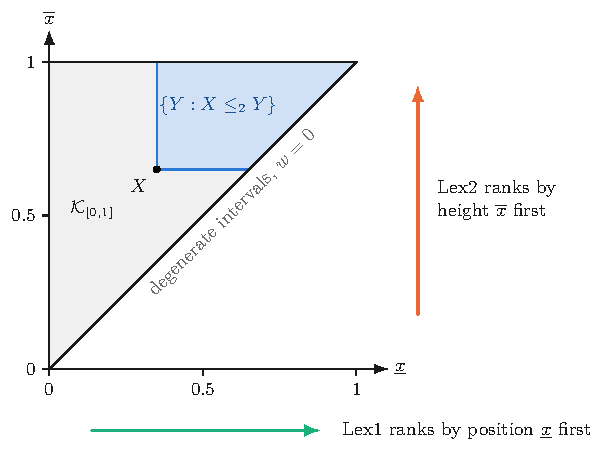
\includegraphics{Figure_1}
\caption{Intervals as points of the plane. An interval $X=[\lo x,\up x]$ is the point $(\lo x,\up x)$ on or above the diagonal, and the shaded region contains the intervals that lie above $X$ in the product order. Lex2 ranks intervals by their upper endpoint first, Lex1 by their lower endpoint first.}
\label{fig:triangle}
\end{figure}

\begin{definition}
An order $\preceq$ on $\K$ is \emph{upper-first} if $\up x<\up y$ implies $X\prec Y$, and \emph{lower-first} if $\lo x<\lo y$ implies $X\prec Y$.
\end{definition}

\begin{lemma}[Uniqueness]\label{lem:unique}
Lex2 is the only upper-first admissible order and Lex1 is the only lower-first admissible order.
\end{lemma}

\begin{proof}
Let $\preceq$ be upper-first and admissible, and let $X\ne Y$. If $\up x\ne\up y$, the comparison of $X$ and $Y$ is forced by the upper-first property and agrees with Lex2. If $\up x=\up y$, then $X$ and $Y$ are comparable in $\le_2$: $X\le_2Y$ if $\lo x\le\lo y$ and $Y\le_2X$ otherwise. Admissibility forces $\preceq$ to agree with $\le_2$, hence with Lex2, which breaks ties in the upper endpoint by the lower endpoint. So $\preceq$ coincides with Lex2 on every pair. Conversely Lex2 is admissible by \Cref{cor:abdef} and upper-first by definition. The statement for Lex1 is symmetric.
\end{proof}

% =====================================================================
\section{Interval networks and soundness}
\label{sec:networks}

We model a network as a composition $f=f_L\circ\cdots\circ f_1$ of real layers acting on tensors, and an \emph{interval network} as a composition $\mathcal N=F_L\circ\cdots\circ F_1$ of interval layers acting on boxes (tensors of intervals). A layer $F$ is \emph{enclosing} for $f$ if $f(B)\subseteq F(B)$ for every box $B$, where $f(B)$ is the image set.

\begin{lemma}[Standard enclosing layers]\label{lem:layers}
The following interval layers are enclosing.
\begin{enumerate}[label=(\alph*)]
\item \emph{Affine maps.} For $f(x)=Wx+b$, $F(\langle c,r\rangle)=\langle Wc+b,\ \abs Wr\rangle$, with $\abs W$ the entrywise absolute value. This covers fully connected and convolutional layers, and BatchNorm in evaluation mode.
\item \emph{Monotone activations.} For non-decreasing $\sigma$ applied coordinate-wise (e.g.\ ReLU), $F([\lo x,\up x])=[\sigma(\lo x),\sigma(\up x)]$.
\item \emph{Average pooling} and any linear map with non-negative weights, applied to both endpoints.
\item \emph{Lattice max-pooling} $M(X_1,\dots,X_p)=X_1\vee\cdots\vee X_p$.
\end{enumerate}
Moreover (a), (b) and (d) are inclusion-isotone, and (a) is exact coordinate-wise: each output coordinate's interval equals the range of that coordinate.
\end{lemma}

\begin{proof}
(a) For $x=c+\delta$ with $\abs\delta\le r$, $\abs{(Wx+b)-(Wc+b)}_k=\abs{\sum_jW_{kj}\delta_j}\le\sum_j\abs{W_{kj}}r_j$. Coordinate $k$ attains $\pm(\abs Wr)_k$ at $\delta_j=\pm r_j\operatorname{sign}W_{kj}$. Isotonicity: if $\langle c,r\rangle\subseteq\langle c',r'\rangle$ then $\abs{c-c'}\le r'-r$ coordinate-wise, so $\abs{W(c-c')}\le\abs W(r'-r)$, which is the inclusion of the outputs. (b) $\sigma$ maps $[\lo x,\up x]$ into $[\sigma(\lo x),\sigma(\up x)]$, and the endpoints are attained; isotonicity follows from monotonicity of $\sigma$. (c) is a special case of (a) with $W\ge0$. (d) follows from \Cref{prop:lattice} below and from monotonicity of $\max$.
\end{proof}

\begin{theorem}[Soundness of compositions]\label{thm:net}
If every layer of $\mathcal N$ is enclosing for the corresponding real layer, then $f(B)\subseteq\mathcal N(B)$ for every input box $B$. Inclusion isotonicity of the layers is not required.
\end{theorem}

\begin{proof}
By induction on $L$. The case $L=1$ is the hypothesis. Let $g=f_{L-1}\circ\cdots\circ f_1$ and $G=F_{L-1}\circ\cdots\circ F_1$ with $g(B)\subseteq G(B)$. Then
\[
f_L(g(B))\subseteq f_L(G(B))\subseteq F_L(G(B)),
\]
where the first inclusion holds because taking images preserves inclusion of sets and the second because $F_L$ is enclosing on the box $G(B)$.
\end{proof}

\begin{corollary}[Certification]\label{cor:cert}
Let $\mathcal N(B)=[\lo z,\up z]$ for a classifier with logits $z$. If $\lo z_y>\max_{k\ne y}\up z_k$, then $\arg\max_kz_k(x')=y$ for every $x'\in B$.
\end{corollary}

\begin{proof}
For $x'\in B$, \Cref{thm:net} gives $z(x')\in[\lo z,\up z]$, so $z_y(x')\ge\lo z_y>\up z_k\ge z_k(x')$ for every $k\ne y$.
\end{proof}

\Cref{cor:cert} is the reason enclosure matters: if a single layer is not enclosing, the inequality $\lo z_y>\max_{k\ne y}\up z_k$ no longer certifies anything.

% =====================================================================
\section{Characterization of enclosing max- and min-pooling}
\label{sec:char}

For a finite family $X=(X_1,\dots,X_p)$ in $\K$, define the ranges of the maximum and of the minimum over the box $\prod_iX_i$:
\[
R_{\max}(X)=\{\max_ix_i:\ x_i\in X_i\},\qquad R_{\min}(X)=\{\min_ix_i:\ x_i\in X_i\}.
\]

\begin{proposition}\label{prop:lattice}
For every family,
\[
R_{\max}(X)=[\max_i\lo x_i,\ \max_i\up x_i]=M(X),\qquad R_{\min}(X)=[\min_i\lo x_i,\ \min_i\up x_i].
\]
Consequently the lattice maximum $M$ is the smallest enclosing max-pooling operator, and it is $1$-Lipschitz for $d$.
\end{proposition}

\begin{proof}
The function $x\mapsto\max_ix_i$ is continuous and non-decreasing in each coordinate on the compact connected box $\prod_iX_i$. Its range is therefore an interval whose endpoints are its values at the lowest corner $(\lo x_i)_i$ and at the highest corner $(\up x_i)_i$. The same argument applies to the minimum. Any enclosing operator must contain $R_{\max}(X)=M(X)$, so $M$ is the smallest. For the Lipschitz bound use $\abs{\max_ia_i-\max_ib_i}\le\max_i\abs{a_i-b_i}$ for each endpoint.
\end{proof}

A \emph{selection operator} is a map $S$ that returns one of its arguments: $S(X)\in\{X_1,\dots,X_p\}$. The admissible maximum $M_\preceq(X)$ (the $\preceq$-largest $X_i$) and the admissible minimum $m_\preceq(X)$ (the $\preceq$-smallest $X_i$) are selection operators.

\begin{lemma}\label{lem:selection}
A selection operator $S$ encloses the maximum if and only if, for every family, the selected interval has the largest upper endpoint: $\up x_{S}=\max_i\up x_i$. It encloses the minimum if and only if the selected interval has the smallest lower endpoint.
\end{lemma}

\begin{proof}
Let $S(X)=X_j$. By \Cref{prop:lattice}, $R_{\max}(X)\subseteq X_j$ if and only if $\lo x_j\le\max_i\lo x_i$ and $\up x_j\ge\max_i\up x_i$. The first inequality always holds; the second is the stated condition. The minimum is symmetric: $R_{\min}(X)\subseteq X_j$ iff $\lo x_j\le\min_i\lo x_i$, since $\up x_j\ge\min_i\up x_i$ always holds.
\end{proof}

\begin{theorem}[Main characterization]\label{thm:char}
For an admissible order $\preceq$ on $\K$ (or on $\K_{[0,1]}$), the following are equivalent:
\begin{enumerate}[label=(\roman*)]
\item the admissible maximum $M_\preceq$ is enclosing;
\item $\preceq$ is upper-first;
\item $\preceq$ is Lex2.
\end{enumerate}
\end{theorem}

\begin{proof}
(ii)$\Leftrightarrow$(iii) is \Cref{lem:unique}.

(ii)$\Rightarrow$(i). Let $X_j=M_\preceq(X)$. If some $X_i$ had $\up x_i>\up x_j$, upper-firstness would give $X_j\prec X_i$, contradicting the maximality of $X_j$. So $\up x_j=\max_i\up x_i$, and \Cref{lem:selection} applies.

(i)$\Rightarrow$(ii). Suppose $\up x<\up y$ but not $X\prec Y$. Since $\preceq$ is total and $X\ne Y$, $Y\prec X$ and $M_\preceq(X,Y)=X$. The selected interval does not have the largest upper endpoint, so by \Cref{lem:selection} $M_\preceq$ is not enclosing. Concretely, $\max(x,y)$ with $y=\up y$ lies outside $X$.
\end{proof}

\begin{corollary}\label{cor:ab}
For an $(\alpha,\beta)$-order, $M_{\preceq_{\alpha,\beta}}$ is enclosing if and only if $\alpha=1$; all orders $\preceq_{1,\beta}$, $\beta<1$, coincide with Lex2. In particular Lex1 and Xu--Yager are not enclosing for max-pooling.
\end{corollary}

\begin{proof}
If $\alpha=1$, the first key is $K_1(X)=\up x$ and ties are broken by $K_\beta(X)=(1-\beta)\lo x+\beta\up x$; with $\up x$ fixed and $\beta<1$ this is increasing in $\lo x$, so the order is Lex2. If $\alpha<1$, choose $t\in(\alpha,1)$, $X=[t,t]$ and $Y=[0,1]$. Then $\up x<\up y$, but $K_\alpha(X)=t>\alpha=K_\alpha(Y)$ gives $Y\prec X$; the order is not upper-first.
\end{proof}

\begin{theorem}[Dual characterization for min-pooling]\label{thm:min}
For an admissible order $\preceq$, the admissible minimum $m_\preceq$ is enclosing for the minimum if and only if $\preceq$ is lower-first, if and only if $\preceq$ is Lex1. Among $(\alpha,\beta)$-orders this means $\alpha=0$.
\end{theorem}

\begin{proof}
By \Cref{lem:selection}, $m_\preceq$ is enclosing iff the $\preceq$-smallest interval always has the smallest lower endpoint. If $\preceq$ is lower-first and $X_j=m_\preceq(X)$ had $\lo x_j>\lo x_i$ for some $i$, then $X_i\prec X_j$, a contradiction. Conversely, if $\lo x<\lo y$ but $Y\prec X$, then $m_\preceq(X,Y)=Y$ does not have the smallest lower endpoint. Uniqueness is \Cref{lem:unique}. For $(\alpha,\beta)$-orders, $\alpha=0$ makes $K_0(X)=\lo x$ the first key, and for $\alpha>0$ the pair $X=[0,1]$, $Y=[t,t]$ with $t\in(0,\alpha)$ has $\lo x<\lo y$ but $K_\alpha(X)=\alpha>t=K_\alpha(Y)$.
\end{proof}

\begin{corollary}[Impossibility]\label{cor:impossible}
No admissible order makes both the admissible maximum and the admissible minimum enclosing. The Xu--Yager order makes neither enclosing.
\end{corollary}

\begin{proof}
By \Cref{thm:char,thm:min} such an order would equal both Lex2 and Lex1, but $[0,1]\prec_{\mathrm{Lex1}}[0.5,0.5]$ while $[0.5,0.5]\prec_{\mathrm{Lex2}}[0,1]$. Xu--Yager is $\preceq_{1/2,1}$, so $\alpha=1/2\notin\{0,1\}$.
\end{proof}

\begin{table}[t]
\centering
\caption{Enclosure status of the admissible maximum and minimum for common orders.}
\label{tab:status}
\begin{tabular}{lccc}
\toprule
Order & First key & Max enclosing & Min enclosing \\
\midrule
Lex1 $=\preceq_{0,1}$ & $\lo x$ & no & yes \\
Lex2 $=\preceq_{1,0}$ & $\up x$ & yes & no \\
Xu--Yager $=\preceq_{1/2,1}$ & $\mathrm{mid}(X)$ & no & no \\
$\preceq_{\alpha,\beta}$, $0<\alpha<1$ & $K_\alpha(X)$ & no & no \\
\bottomrule
\end{tabular}
\end{table}

\begin{example}\label{ex:fail}
Lex1 with $X_1=[0.5,0.5]$ and $X_2=[0.4,1]$ selects $X_1$ because $0.5>0.4$; choosing $x_2=0.9$ gives $\max(x_1,x_2)=0.9\notin X_1$. Xu--Yager with $X_1=[0.5,0.5]$ and $X_2=[0,0.9]$ selects $X_1$ because its midpoint $0.5$ exceeds $0.45$; again $x_2=0.9$ violates enclosure.
\end{example}

% =====================================================================
\section{The price and the regularity of sound admissible pooling}
\label{sec:price}

By \Cref{thm:char}, from now on the only admissible order of interest for max-pooling is Lex2, and we write $M_2=M_{\mathrm{Lex2}}$.

\subsection{Excess width}

\begin{proposition}[Excess width]\label{prop:excess}
Let $X_j=M_2(X)$ and $e(X)=w(M_2(X))-w(M(X))$. Then
\[
e(X)=\max_i\lo x_i-\lo x_j,\qquad 0\le e(X)\le w(X_j).
\]
Moreover $e(X)=0$ if and only if the family has a $\le_2$-greatest element, i.e.\ $M(X)\in\{X_1,\dots,X_p\}$, and the upper bound is sharp: $\sup e(X)/w(M_2(X))=1$ over families with $w(M_2(X))>0$.
\end{proposition}

\begin{proof}
By \Cref{thm:char}, $\up x_j=\max_i\up x_i$, so $M_2(X)$ and $M(X)$ share their upper endpoint and $e(X)=\max_i\lo x_i-\lo x_j\ge0$. For every $i$, $\lo x_i\le\up x_i\le\up x_j$, hence $\max_i\lo x_i\le\up x_j$ and $e(X)\le w(X_j)$. If $e(X)=0$ then $X_j=M(X)$ is $\le_2$-greatest; conversely a $\le_2$-greatest element is Lex2-greatest because Lex2 refines $\le_2$. For sharpness take $X_1=[0,1]$ and $X_2=[1-\delta,1-\delta]$, $\delta\in(0,1)$: Lex2 selects $X_1$, $e=1-\delta$ and $w(X_1)=1$.
\end{proof}

\subsection{Comparison of networks}

\begin{lemma}[Mixed isotonicity]\label{lem:mixed}
If $X_i\subseteq Y_i$ for all $i$, then $M(X)\subseteq M_2(Y)$.
\end{lemma}

\begin{proof}
Let $Y_j=M_2(Y)$. Its upper endpoint is $\max_i\up y_i\ge\max_i\up x_i$. Its lower endpoint satisfies $\lo y_j\le\lo x_j\le\max_i\lo x_i$ because $X_j\subseteq Y_j$. Hence $M(X)=[\max_i\lo x_i,\max_i\up x_i]\subseteq Y_j$.
\end{proof}

\begin{theorem}[Lattice networks are never wider]\label{thm:compare}
Let $\mathcal N_{\mathrm{lat}}$ and $\mathcal N_2$ be two interval networks that differ only in their max-pooling layers, which use $M$ and $M_2$ respectively, and suppose all other layers are inclusion-isotone (\Cref{lem:layers}). Then $\mathcal N_{\mathrm{lat}}(B)\subseteq\mathcal N_2(B)$ for every box $B$, for any number of pooling layers.
\end{theorem}

\begin{proof}
We show by induction on the layer index that the intermediate boxes satisfy $B^{\mathrm{lat}}_\ell\subseteq B^{(2)}_\ell$. Both start from $B$. If layer $\ell$ is not a pooling layer it is the same isotone map in both networks, and the inclusion is preserved. If it is a pooling layer, each window of $B^{\mathrm{lat}}_{\ell-1}$ is contained window-wise in the corresponding window of $B^{(2)}_{\ell-1}$, and \Cref{lem:mixed} gives the inclusion of the outputs.
\end{proof}

\begin{example}\label{ex:strict}
The inclusion is strict in general: for the family $X_1=[0,1]$, $X_2=[0.8,0.9]$, $M(X)=[0.8,1]$ while $M_2(X)=[0,1]$, and a following ReLU or affine layer with non-zero weight preserves the gap.
\end{example}

\subsection{Isotonicity and continuity}

\begin{theorem}\label{thm:not-isotone}
$M_2$ is not inclusion-isotone.
\end{theorem}

\begin{proof}
Let $X_1=[0.4,0.5]$, $X_2=[0,0.6]$, $Y_1=[0.4,0.7]$, $Y_2=[0,0.6]$; then $X_i\subseteq Y_i$. Lex2 selects the larger upper endpoint, so $M_2(X)=X_2=[0,0.6]$ and $M_2(Y)=Y_1=[0.4,0.7]$, and $[0,0.6]\not\subseteq[0.4,0.7]$.
\end{proof}

\begin{remark}
\Cref{thm:not-isotone} shows that the enclosure of $M_2$ cannot be obtained from \Cref{thm:fund}; it follows from the direct argument of \Cref{thm:char}, and soundness of networks follows from \Cref{thm:net}, which does not need isotonicity.
\end{remark}

\begin{proposition}\label{prop:discont}
$M_2$ is not continuous with respect to $d$; more precisely, it has jumps of size arbitrarily close to $1$ on $\K_{[0,1]}$.
\end{proposition}

\begin{proof}
Let $X_1=[0,1]$ and $X_2^\delta=[1-\eta,1-\delta]$ for fixed $\eta\in(0,1)$ and $\delta\in[0,\eta)$. For $\delta>0$, Lex2 selects $X_1=[0,1]$. For $\delta=0$, the upper endpoints tie and $X_1\le_2X_2^0$, so Lex2 selects $X_2^0=[1-\eta,1]$. As $\delta\to0$ the input moves by $\delta$ in $d$, while the output jumps by $d([0,1],[1-\eta,1])=1-\eta$.
\end{proof}

\subsection{Gradients}

\begin{proposition}\label{prop:grad}
Assume the maximizers are unique. Then
\[
\frac{\partial\,\lo M(X)}{\partial\lo x_i}=\mathbf 1[i=\arg\max_k\lo x_k],\qquad
\frac{\partial\,\up M(X)}{\partial\up x_i}=\mathbf 1[i=\arg\max_k\up x_k],
\]
whereas for $M_2$, with $j=\arg\max_k\up x_k$,
\[
\frac{\partial\,\lo M_2(X)}{\partial\lo x_i}=\frac{\partial\,\up M_2(X)}{\partial\up x_i}=\mathbf 1[i=j],
\]
and all other partial derivatives vanish.
\end{proposition}

\begin{proof}
Under uniqueness, each selected index is locally constant, so the outputs are locally coordinate projections.
\end{proof}

In words, the lattice maximum can send the gradients of the two endpoints to different inputs, while the Lex2 maximum sends both to the input with the largest upper endpoint. In IBP training the lower endpoint of the true-class logit is pushed up; under Lex2 this signal reaches only the window element with the largest upper bound, which need not be the one with the largest lower bound.

\subsection{How often unsound selections fail}

Empirical soundness tests sample points from the input box and check whether outputs fall inside the computed bounds. The following formula predicts the outcome at a single pooling window.

\begin{proposition}[Violation probability]\label{prop:violation}
Let $S$ select $X_j$ from a family with $w(X_i)>0$ for all $i\ne j$, and let $x_i\sim\mathrm{Unif}(X_i)$ be independent. Then
\[
\Pr\big[\max_ix_i\notin X_j\big]=1-\prod_{i\ne j}\min\Big(1,\ \max\Big(0,\frac{\up x_j-\lo x_i}{w(X_i)}\Big)\Big).
\]
For two intervals selected by Lex1 with $\lo x_1>\lo x_2$ and $\up x_2>\up x_1$, this equals $(\up x_2-\up x_1)/w(X_2)$.
\end{proposition}

\begin{proof}
Since $\max_ix_i\ge x_j\ge\lo x_j$, the only way to leave $X_j$ is $\max_ix_i>\up x_j$, i.e.\ some $x_i>\up x_j$ with $i\ne j$ (as $x_j\le\up x_j$). By independence, $\Pr[\text{all }x_i\le\up x_j]=\prod_{i\ne j}\Pr[x_i\le\up x_j]$, and $\Pr[x_i\le t]=\min(1,\max(0,(t-\lo x_i)/w(X_i)))$. In the two-interval case $\lo x_2<\lo x_1\le\up x_1<\up x_2$, so $\Pr[x_2\le\up x_1]=(\up x_1-\lo x_2)/w(X_2)$ and the complement is $(\up x_2-\up x_1)/w(X_2)$.
\end{proof}

\begin{remark}
\Cref{prop:violation} shows that violations are not rare corner cases: in \Cref{ex:fail} the Lex1 violation probability is $0.5/0.6\approx0.83$. Sampling-based soundness checks will therefore detect unsound pooling quickly, which makes the predictions of \Cref{thm:char} directly testable.
\end{remark}

\subsection{A worked example on one pooling window}

\Cref{fig:window} shows a $2\times2$ window with intervals
\[
X_1=[0.10,0.95],\quad X_2=[0.55,0.70],\quad X_3=[0.60,0.62],\quad X_4=[0.20,0.40].
\]
The range of the maximum is $M(X)=[0.60,0.95]$. The four operators give:
\begin{itemize}
\item \emph{Lattice:} $[0.60,0.95]$, exact.
\item \emph{Lex2:} selects $X_1$ (largest upper endpoint), output $[0.10,0.95]$; enclosing, with excess width $e=0.60-0.10=0.50$ (\Cref{prop:excess}).
\item \emph{Lex1:} selects $X_3$ (largest lower endpoint), output $[0.60,0.62]$; not enclosing. With $\up x_3=0.62$, \Cref{prop:violation} gives $\Pr[x_1\le0.62]=0.52/0.85$, $\Pr[x_2\le0.62]=0.07/0.15$ and $\Pr[x_4\le0.62]=1$, so the violation probability is $1-(0.52/0.85)(0.07/0.15)\approx0.71$.
\item \emph{Xu--Yager:} the midpoints are $0.525$, $0.625$, $0.61$ and $0.30$, so it selects $X_2=[0.55,0.70]$; not enclosing. With $\up x_2=0.70$, only $X_1$ can exceed it, and the violation probability is $1-0.60/0.85\approx0.29$.
\end{itemize}

\begin{figure}[t]
\centering
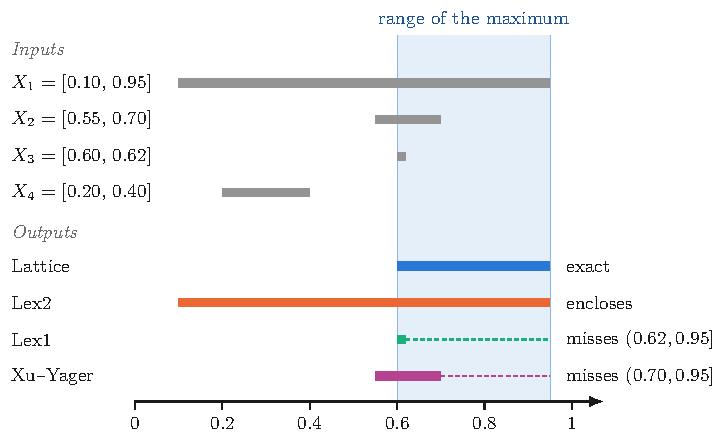
\includegraphics{Figure_2}
\caption{One $2\times2$ pooling window. The four input intervals, the range of the maximum (shaded band), and the outputs of the lattice maximum and of the three admissible maxima. A dashed segment marks the part of the range that an unsound output misses.}
\label{fig:window}
\end{figure}

\subsection{Beyond the maximum: rank pooling}

Median and other rank-based pooling select the $k$-th largest element. For a family $X$ of $p$ intervals let $L_{(k)}$ and $U_{(k)}$ denote the $k$-th largest lower and upper endpoints.

\begin{proposition}\label{prop:rank}
The range of the $k$-th largest coordinate over $\prod_iX_i$ is $[L_{(k)},U_{(k)}]$. For $p=3$ and $k=2$, neither the second element in Lex2 nor the second element in Lex1 is enclosing.
\end{proposition}

\begin{proof}
The $k$-th largest coordinate is continuous and non-decreasing in each coordinate, so its range over the connected box is the interval between its values at the lowest and the highest corners, which are $L_{(k)}$ and $U_{(k)}$. For Lex2 take $X_1=[0,1]$, $X_2=[0.9,0.95]$, $X_3=[0.8,0.85]$: the second element is $X_2$, but the range is $[0.8,0.95]\not\subseteq X_2$. For Lex1 take $X_1=[0,1]$, $X_2=[0.5,0.55]$, $X_3=[0.6,0.65]$: the second element is $X_2$, but the range is $[0.5,0.65]\not\subseteq X_2$.
\end{proof}

\begin{question}
Characterize the selection rules that enclose the $k$-th largest coordinate for $1<k<p$. By \Cref{prop:rank} they cannot be ``$k$-th element of Lex1 or Lex2''; the endpoint-wise rule $[L_{(k)},U_{(k)}]$ is exact but is not a selection.
\end{question}

% =====================================================================
\section{Endpoint-wise pooling with aggregation functions}
\label{sec:agg}

Aggregation-based pooling \cite{rodriguez2022,rodriguez2023,forcen2020} suggests a second family of interval pooling operators that act on the two endpoints separately. An \emph{aggregation function} is a map $G:[0,1]^p\to[0,1]$ that is non-decreasing in each argument with $G(0,\dots,0)=0$ and $G(1,\dots,1)=1$. It is \emph{averaging} if $\min_ia_i\le G(a)\le\max_ia_i$ and \emph{disjunctive} if $G(a)\ge\max_ia_i$. For aggregation functions $A,B$ with $A\le B$ pointwise, define
\[
P_{A,B}(X)=\big[A(\lo x_1,\dots,\lo x_p),\ B(\up x_1,\dots,\up x_p)\big].
\]
This is an interval, because $A(\lo x)\le A(\up x)\le B(\up x)$ by monotonicity of $A$ and $A\le B$.

\begin{theorem}\label{thm:agg}
$P_{A,B}$ is enclosing for the maximum if and only if $A(a)\le\max_ia_i$ and $B(b)\ge\max_ib_i$ for all $a,b\in[0,1]^p$. In particular:
\begin{enumerate}[label=(\alph*)]
\item if $B$ is averaging, $P_{A,B}$ is enclosing iff $B=\max$ and $A(a)\le\max_ia_i$;
\item if $A$ is averaging and $B$ is disjunctive, $P_{A,B}$ is enclosing;
\item among enclosing $P_{A,B}$, the lattice maximum ($A=B=\max$) is the smallest, and $P_{A,B}=M$ iff $A=B=\max$.
\end{enumerate}
\end{theorem}

\begin{proof}
By \Cref{prop:lattice}, enclosure means $A(\lo x)\le\max_i\lo x_i$ and $B(\up x)\ge\max_i\up x_i$ for every family. Every vector of $[0,1]^p$ occurs as a vector of lower endpoints (take $\up x_i=1$) and as a vector of upper endpoints (take degenerate intervals), which gives the condition. (a) If $B$ is averaging then $B\le\max$, so $B\ge\max$ forces $B=\max$. (b) Averaging $A$ satisfies $A\le\max$ and disjunctive $B$ satisfies $B\ge\max$. (c) Each enclosing operator contains $M(X)$ by \Cref{prop:lattice}; equality for all families forces $A(a)=\max_ia_i$ and $B(b)=\max_ib_i$ on all of $[0,1]^p$.
\end{proof}

\begin{example}
Ordered weighted averages \cite{forcen2020}, the arithmetic mean and the Choquet integral \cite{bustince2013choquet} are averaging; used as $B$ they are enclosing only when they reduce to the maximum, i.e.\ an OWA with all weight on the largest argument. The probabilistic sum $B(b_1,b_2)=b_1+b_2-b_1b_2$ is disjunctive and enclosing, but strictly wider than the lattice maximum whenever both arguments lie in $(0,1)$.
\end{example}


% =====================================================================
\section{Method}
\label{sec:method}

\paragraph{Representation} Interval feature maps are stored in center--radius form $\langle c,r\rangle$ with $r\ge0$, and converted to endpoints $(c-r,c+r)$ only inside pooling layers.

\paragraph{Interval layers} Convolutions and linear layers use \Cref{lem:layers}(a) with the same kernel for centers and radii; ReLU uses \Cref{lem:layers}(b). BatchNorm in training mode normalizes both the clean pass and the interval pass with the statistics of the clean batch, and updates its running statistics only from the clean pass \cite{shi2021,ioffe2015}; the affine map is then fixed per batch, so \Cref{lem:layers}(a) applies.

\paragraph{Pooling operators} For a $k\times k$ window with endpoints $(\lo x_i,\up x_i)_{i=1}^{k^2}$ obtained by unfolding the feature map:
\begin{enumerate}[leftmargin=*]
\item \emph{Lattice:} $[\max_i\lo x_i,\max_i\up x_i]$, implemented as two max-pooling calls.
\item \emph{Lex2:} compute $u^*=\max_i\up x_i$; restrict to $T=\{i:\up x_i\ge u^*-\tau\}$ with a tolerance $\tau$ for floating-point ties; select $j=\arg\max_{i\in T}\lo x_i$; output $X_j$ by gathering both endpoints at index $j$.
\item \emph{Lex1:} the same with the roles of the endpoints exchanged.
\item \emph{Xu--Yager:} first key $\mathrm{mid}(X_i)$, ties broken by $\up x_i$.
\end{enumerate}
Each selection costs two reductions over the window and one gather, i.e.\ $O(k^2)$ per output, the same order as standard max-pooling. Gradients flow through the gathered endpoints as described in \Cref{prop:grad}. We use $\tau=10^{-6}$. The selected upper endpoint can then fall below $u^*$ by at most $\tau$, so enclosure holds up to $\tau$, which is below the $10^{-5}$ threshold of the soundness test; returning $[\lo x_j,u^*]$ instead would remove this gap.

\paragraph{Architecture} The reference is CNN-7 \cite{shi2021}: five $3\times3$ convolutions with $64$, $64$, $128$, $128$ and $128$ channels, the third with stride 2, a hidden linear layer of width 512 and the output layer, each hidden layer followed by BatchNorm and ReLU. In the pooled variant (pool1) the stride-2 convolution is replaced by a stride-1 convolution followed by $2\times2$ pooling with stride 2, so that the model has exactly one pooling layer. In a second variant (pool2), which tests \Cref{thm:compare} with more than one pooling layer, a further $2\times2$ pooling layer with stride 2 follows the second convolution. The third convolution then runs at half the input resolution and the last two at a quarter, and the input of the hidden linear layer is four times smaller, so pool2 has $3.6$ million parameters on MNIST and $4.6$ million on CIFAR-10, against $13.3$ and $17.2$ million for pool1. Both pooling layers of a network use the same operator.

\paragraph{Training} We use the IBP recipe of \citet{shi2021}, which is also the IBP baseline of CTBench \cite{mao2024ctbench}, so that the unmodified CNN-7 can be compared with published numbers. The loss is the cross-entropy of the negated margin bounds, $\mathrm{CE}(-m,y)$, where $m_j$ is a lower bound of $f_y-f_j$ over the box and the last linear layer is applied to $w_y-w_j$ directly; this is exact for that layer, tighter than subtracting logit intervals, and still sound. No clean term is mixed in once $\eps>0$. Weights use the IBP initialization. $\eps$ follows the smoothed schedule of \citet{gowal2018}, proportional to $t^4$ for the first quarter of the ramp and then linear; the ramp takes 20 epochs on MNIST and 80 on CIFAR-10, the latter after one clean epoch. During the ramp we add $\lambda(\mathcal L_{\mathrm{tightness}}+\mathcal L_{\mathrm{relu}})$ with $\lambda=(1-\eps/\eps_{\mathrm{target}})/2$ and tolerance $1/2$ \cite{shi2021}. Adam with learning rate $5\cdot10^{-4}$, decayed by $0.2$ at epochs 50 and 60 of 70 on MNIST and 120 and 140 of 160 on CIFAR-10; gradient clipping at $10$; batch size 256 on MNIST and 128 on CIFAR-10. MNIST inputs are not normalized or augmented. CIFAR-10 inputs are normalized per channel, with random horizontal flips and random crops with 2 pixels of edge padding.

\paragraph{Soundness test} For each of the first $500$ test images we sample $120$ points of the input box: $100$ uniform points and $20$ random corners. At each point we compute the real network and compare it with the computed intervals at two levels. A \emph{logit violation} is an (input, logit) pair whose sampled value leaves the logit interval by more than $10^{-5}$. A \emph{window violation} is a window of the first pooling layer whose true maximum at some sampled point leaves the pooled interval by more than $10^{-4}$; this is the quantity of \Cref{prop:violation}. In pool2 the first pooling layer is the one after the second convolution; the second pooling layer is covered only by the logit test. Both rates are lower bounds on the true rates, since sampling can miss violations.

\paragraph{Metrics}
\begin{itemize}
\item window and logit violation rates, and the largest excess of a window maximum over its interval (all operators);
\item clean accuracy (all operators);
\item verified accuracy via \Cref{cor:cert}, computed on the margin bounds and reported only for enclosing operators;
\item mean output width of the predicted logit, and the width ratio to the lattice network;
\item training time per epoch.
\end{itemize}

% =====================================================================
\section{Experimental protocol and hypotheses}
\label{sec:protocol}

\paragraph{Datasets} The standard benchmarks of certified training \cite{shi2021,mao2024ctbench}: MNIST \cite{lecun1998} with $\eps\in\{0.1,0.3\}$ and CIFAR-10 \cite{krizhevsky2009} with $\eps\in\{2/255,8/255\}$. The training radius equals the test radius. As in those works models train on the full training split; we evaluate the final epoch, with no selection on test data, and the test set is used once. Fashion-MNIST \cite{xiao2017fmnist} runs from an earlier version of the training recipe are reported in \Cref{sec:fmnist} as supplementary results only.

\paragraph{Repetitions} Three seeds per configuration. We report means with 95\% confidence intervals from the $t$-distribution, and paired comparisons between pooling operators on the same seed.

\paragraph{Hypotheses} Each is a direct prediction of the theory.
\begin{itemize}
\item[\textbf{H1}] The violation rate is $0$ for the lattice maximum and for Lex2 (\Cref{thm:char,lem:layers}).
\item[\textbf{H2}] The violation rate is positive for Lex1 and Xu--Yager, of the magnitude suggested by \Cref{prop:violation}.
\item[\textbf{H3}] The width ratio Lex2/lattice is at least $1$ (\Cref{thm:compare}), and its excess is bounded as in \Cref{prop:excess}.
\item[\textbf{H4}] Verified accuracy with Lex2 is at most that of the lattice network with the same weights; after training, the gap measures how much the network adapts to the coarser operator.
\item[\textbf{H5}] Training with Lex2 is less stable than with the lattice maximum, because of the discontinuity (\Cref{prop:discont}) and the gradient routing (\Cref{prop:grad}).
\end{itemize}

\paragraph{Compute} All runs used a single NVIDIA GeForce GTX 1660 Ti. An IBP epoch on MNIST takes about $50$\,s for the unmodified CNN-7 and $64$--$73$\,s for the pooled variant with either sound operator (about $23$\,s without IBP), so a $70$-epoch run takes $1$--$1.4$\,h. On CIFAR-10 an epoch takes about $73$\,s without pooling and $100$--$120$\,s with one pooling layer (about $28$\,s without IBP), so a $160$-epoch pooled run takes $4.5$--$5.5$\,h. The pool1 network is slower because its third convolution runs at full resolution. With two pooling layers an IBP epoch takes $48$--$51$\,s on MNIST and $54$--$58$\,s on CIFAR-10, half as long as pool1, so a run takes $0.8$--$1$\,h and $2.2$--$2.6$\,h respectively. All training runs of this paper took about $161$ GPU-hours, $40$ of them for pool2, and the evaluations of \Cref{tab:main,tab:main-pool2} under $4$ more. We therefore train only the two sound operators (Lex1 and Xu--Yager are evaluated on the same weights) and use three seeds.

% =====================================================================
\section{Results}
\label{sec:results}

\subsection{Checking the training recipe}

The unmodified CNN-7 was trained with the recipe of \Cref{sec:method} and compared with published IBP results (\Cref{tab:ref}): the original numbers of \citet{shi2021}, and those of CTBench \cite{mao2024ctbench}, which reruns the same recipe with tuned hyperparameters. Against \citet{shi2021}, our verified accuracy is within $0.15$ points at MNIST $0.3$ and CIFAR-10 $2/255$. It is $1.05$ points lower at CIFAR-10 $8/255$ and $1.44$ points lower at MNIST $0.1$. CTBench, with tuned hyperparameters, is $0.3$ to $3.1$ points above \citet{shi2021}. We have not found the cause of the gap at MNIST $0.1$, where our clean accuracy is the highest of the three. Every model trained at a given radius uses the same recipe, so these gaps do not affect the comparison between pooling operators.

\begin{table}[ht]
\centering\small
\setlength{\tabcolsep}{4pt}
\caption{Unmodified CNN-7 (stride-2 convolution, no pooling) trained with IBP: clean and verified test accuracy (\%), ours as mean $\pm$ standard deviation over three seeds, against the IBP results of \citet{shi2021} and of CTBench \cite{mao2024ctbench} (one number each). Bold: best per row and metric.}
\label{tab:ref}
\begin{tabular}{lcccccc}
\toprule
 & \multicolumn{2}{c}{Ours} & \multicolumn{2}{c}{\citet{shi2021}} & \multicolumn{2}{c}{CTBench} \\
\cmidrule(lr){2-3}\cmidrule(lr){4-5}\cmidrule(lr){6-7}
Setting & Clean & Verified & Clean & Verified & Clean & Verified \\
\midrule
MNIST $0.1$ & $\mathbf{99.16\pm0.04}$ & $96.51\pm0.14$ & $98.84$ & $97.95$ & $98.87$ & $\mathbf{98.26}$ \\
MNIST $0.3$ & $98.49\pm0.05$ & $93.22\pm0.10$ & $97.67$ & $93.10$ & $\mathbf{98.54}$ & $\mathbf{93.80}$ \\
CIFAR-10 $2/255$ & $67.05\pm0.16$ & $52.83\pm0.15$ & $66.84$ & $52.85$ & $\mathbf{67.49}$ & $\mathbf{55.99}$ \\
CIFAR-10 $8/255$ & $47.87\pm0.38$ & $33.92\pm0.01$ & $\mathbf{48.94}$ & $34.97$ & $48.51$ & $\mathbf{35.28}$ \\
\bottomrule
\end{tabular}
\end{table}

\subsection{Training with sound pooling}

\Cref{tab:train} gives the pooled CNN-7 with one and with two pooling layers, trained with the lattice maximum and with Lex2, next to the unmodified CNN-7 and a normally trained pooled network. Each IBP network is evaluated with the operator it was trained with.

\begin{table}[ht]
\centering\small
\setlength{\tabcolsep}{4pt}
\caption{Clean and verified test accuracy (\%) at the training radius, mean $\pm$ standard deviation over three seeds. ``Pooled'' has one pooling layer (pool1), ``Pooled $\times2$'' two (pool2). ``Standard'' is the pool1 network trained without IBP. Bold: best among the IBP-trained models.}
\label{tab:train}
\begin{tabular}{lcccc}
\toprule
\multicolumn{5}{l}{\emph{MNIST}} \\
 & \multicolumn{2}{c}{$\eps=0.1$} & \multicolumn{2}{c}{$\eps=0.3$} \\
\cmidrule(lr){2-3}\cmidrule(lr){4-5}
Model & Clean & Verified & Clean & Verified \\
\midrule
CNN-7, no pooling & $\mathbf{99.16\pm0.04}$ & $96.51\pm0.14$ & $\mathbf{98.49\pm0.05}$ & $\mathbf{93.22\pm0.10}$ \\
Pooled, lattice   & $99.06\pm0.03$ & $96.45\pm0.04$ & $98.43\pm0.09$ & $93.03\pm0.16$ \\
Pooled, Lex2      & $99.10\pm0.04$ & $96.46\pm0.07$ & $98.24\pm0.04$ & $92.57\pm0.18$ \\
Pooled $\times2$, lattice & $98.85\pm0.06$ & $\mathbf{96.74\pm0.04}$ & $97.72\pm0.17$ & $91.66\pm0.21$ \\
Pooled $\times2$, Lex2    & $98.94\pm0.02$ & $96.62\pm0.12$ & $96.98\pm0.09$ & $89.34\pm0.48$ \\
Pooled, standard  & $99.56\pm0.04$ & $0.00$ & $99.58\pm0.02$ & $0.00$ \\
\midrule
\multicolumn{5}{l}{\emph{CIFAR-10}} \\
 & \multicolumn{2}{c}{$\eps=2/255$} & \multicolumn{2}{c}{$\eps=8/255$} \\
\cmidrule(lr){2-3}\cmidrule(lr){4-5}
Model & Clean & Verified & Clean & Verified \\
\midrule
CNN-7, no pooling & $67.05\pm0.16$ & $52.83\pm0.15$ & $47.87\pm0.38$ & $33.92\pm0.01$ \\
Pooled, lattice   & $\mathbf{67.44\pm0.21}$ & $\mathbf{53.08\pm0.64}$ & $\mathbf{48.13\pm0.52}$ & $\mathbf{34.11\pm0.33}$ \\
Pooled, Lex2      & $67.34\pm0.30$ & $52.59\pm0.07$ & $47.14\pm0.65$ & $33.25\pm0.77$ \\
Pooled $\times2$, lattice & $66.69\pm0.23$ & $52.76\pm0.16$ & $47.01\pm0.28$ & $33.33\pm0.27$ \\
Pooled $\times2$, Lex2    & $65.58\pm0.22$ & $52.10\pm0.26$ & $44.03\pm0.97$ & $30.99\pm0.88$ \\
Pooled, standard  & $90.86\pm0.10$ & $0.00$ & $90.98\pm0.10$ & $0.00$ \\
\bottomrule
\end{tabular}
\end{table}

Three observations follow from the networks with one pooling layer.
\begin{enumerate}[leftmargin=*]
\item Sound pooling costs nothing measurable compared with the stride-2 convolution it replaces. With the lattice maximum, verified accuracy is $0.06$ and $0.19$ points lower on MNIST and $0.25$ and $0.19$ points higher on CIFAR-10, all within about one standard deviation.
\item Lex2 is never better than the lattice maximum by more than noise. Paired by seed, lattice minus Lex2 verified accuracy is $-0.01\pm0.08$ points at MNIST $0.1$, $0.46\pm0.69$ at MNIST $0.3$, $0.49\pm1.73$ at CIFAR-10 $2/255$ and $0.86\pm1.26$ at CIFAR-10 $8/255$ (mean and half-width of the 95\% $t$-interval). The direction agrees with \Cref{thm:compare} in three of four settings, but with three seeds none of these intervals excludes $0$.
\item At CIFAR-10 $8/255$ the Lex2 network is also $1.00\pm0.75$ points lower in clean accuracy, the only difference between the two operators whose interval excludes $0$. Training with the coarser operator changes the weights, not only the bounds; we return to this under H4.
\end{enumerate}
The normally trained networks certify nothing at any radius, as expected.

\paragraph{Two pooling layers} With a second pooling layer the picture changes in two ways.
\begin{enumerate}[leftmargin=*]
\item A second sound pooling layer is no longer free at the larger radii. With the lattice maximum, verified accuracy is $0.23$ points above the unmodified CNN-7 at MNIST $0.1$, the best of all models there, and $0.07$ points below it at CIFAR-10 $2/255$. It is $1.55$ points below at MNIST $0.3$ and $0.59$ points below at CIFAR-10 $8/255$. Clean accuracy is lower than with one pooling layer on every benchmark, by $0.21$ to $1.12$ points. The pool2 network also has about a quarter of the parameters of pool1, so this cost cannot be attributed to the pooling operator alone.
\item The gap between the operators widens. Paired by seed, lattice minus Lex2 verified accuracy is $0.11\pm0.22$ points at MNIST $0.1$, $2.33\pm0.89$ at MNIST $0.3$, $0.66\pm0.24$ at CIFAR-10 $2/255$ and $2.34\pm1.68$ at CIFAR-10 $8/255$. All four differences point in the direction of \Cref{thm:compare}, and all but the one at MNIST $0.1$ exclude $0$; with one pooling layer none did. Clean accuracy follows the same pattern, $-0.09\pm0.12$, $0.74\pm0.21$, $1.11\pm0.92$ and $2.98\pm1.74$ points, again with all intervals but the one at MNIST $0.1$ excluding $0$.
\end{enumerate}

\paragraph{Training stability (H5)} \Cref{fig:stability} shows the monitored verified accuracy and the mean gradient norm per epoch. Because the models train on the full training split, the monitored images are training images; they serve only to follow training, not to select a model. We counted the epochs in which monitored verified accuracy fell by more than $2$ points from the previous epoch, summed over the three seeds. At CIFAR-10 $8/255$ there were $7$ such drops with Lex2 and $2$ with the lattice maximum. At $2/255$ there were $1$ and $2$, and the largest drop of all ($15.9$ points, recovered within one epoch) occurred with the lattice maximum. The unpooled CNN-7 had more drops than either pooled network ($6$ at $2/255$ and $8$ at $8/255$). On MNIST no run had such a drop. At MNIST $0.3$ the largest gradient norm of an epoch exceeded the clipping threshold $10$ in $13.7$ epochs on average with the lattice maximum and $9.3$ with Lex2. With two pooling layers (not shown in \Cref{fig:stability}) the count was $2$ drops with Lex2 and $0$ with the lattice maximum at CIFAR-10 $8/255$, and none with either at $2/255$. On MNIST, one lattice run at $\eps=0.3$ fell four times after the end of the ramp, by up to $41.0$ points, and recovered within one or two epochs each time; Lex2 had $2$ smaller drops at $0.3$ and $1$ at $0.1$. The clipping threshold was exceeded in $21.0$ epochs on average with the lattice maximum and $5.0$ with Lex2 at MNIST $0.3$, and in $1.0$ and $7.0$ at CIFAR-10 $8/255$. The evidence for H5 is therefore weak: Lex2 was less smooth only at the largest CIFAR-10 radius, with either number of pooling layers, the lattice maximum was the less smooth one at MNIST $0.3$ with two, and the operator mattered less than whether the network pools at all. The discontinuity of \Cref{prop:discont} occurs only at exact ties of upper endpoints, which appear to be rare in trained networks.

\begin{figure}[p]
\centering
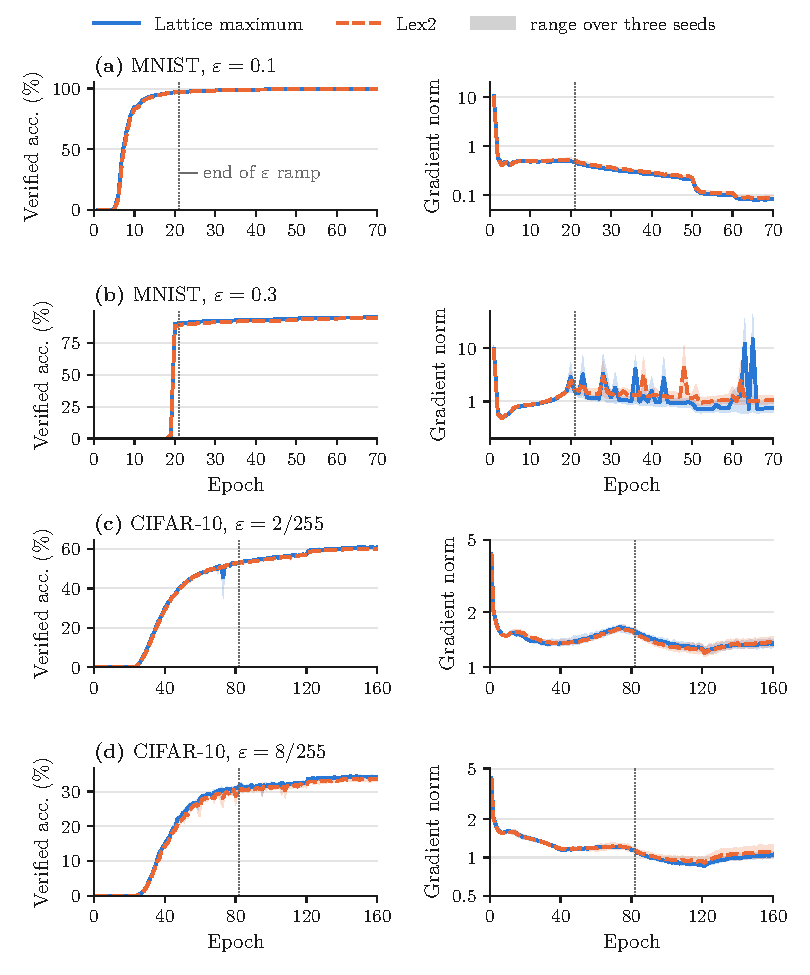
\includegraphics{Figure_3}
\caption{Training of the pooled CNN-7 with one pooling layer. Monitored verified accuracy (left) and mean gradient norm per epoch (right, logarithmic scale) with the lattice maximum and with Lex2. Lines are means over three seeds and bands show the range over the seeds. The dotted vertical line marks the end of the $\eps$ ramp.}
\label{fig:stability}
\end{figure}

\subsection{Pooling operators on the same weights}

\Cref{tab:main} (one pooling layer) and \Cref{tab:main-pool2} (two pooling layers) collect the tests of hypotheses H1--H4, and \Cref{tab:main-fmnist} in \Cref{sec:fmnist} does the same for the Fashion-MNIST networks. Each IBP network of \Cref{tab:train,tab:fmnist} is evaluated again with every pooling operator, without retraining, using the soundness test of \Cref{sec:method}; in pool2 the operator is swapped in both pooling layers. The window threshold $10^{-4}$ is set by floating-point error. In single precision, the sound operators exceed their interval by up to $6.5\cdot10^{-5}$ (column ``max excess''). Recomputed in double precision, the lattice maximum gives no excess and Lex2 gives at most $10^{-6}$, its tie tolerance $\tau$.

% generated by notebooks/A_analysis.ipynb; do not edit by hand
\begin{table}[tbp]
\centering\footnotesize
\setlength{\tabcolsep}{3.5pt}
\caption{Each trained network with one pooling layer evaluated with every pooling operator on the same weights.}
\label{tab:main}
\begin{tabular}{llccccc}
\toprule
Weights & Pooling & Window viol. & Max excess & Logit viol. & Verified & Width ratio \\
\midrule
\multicolumn{7}{l}{\emph{MNIST $0.1$}} \\
\addlinespace[2pt]
Lattice & Lattice & $0$ & $6.5\cdot10^{-5}$ & $0$ & $96.45\pm0.04$ & $1.000$ \\
Lattice & Lex2 & $0$ & $4.7\cdot10^{-5}$ & $0$ & $96.29\pm0.07$ & $1.031$ \\
Lattice & Lex1 & $3.1\cdot10^{-3}$ & $1.2\cdot10^{0}$ & $0$ & n/a & $0.994$ \\
Lattice & Xu--Yager & $2.2\cdot10^{-3}$ & $5.5\cdot10^{-1}$ & $0$ & n/a & $0.999$ \\
Lex2 & Lex2 & $0$ & $3.4\cdot10^{-5}$ & $0$ & $96.46\pm0.07$ & $1.027$ \\
Lex2 & Lattice & $0$ & $3.2\cdot10^{-5}$ & $0$ & $\mathbf{96.66\pm0.10}$ & $1.000$ \\
\midrule
\multicolumn{7}{l}{\emph{MNIST $0.3$}} \\
\addlinespace[2pt]
Lattice & Lattice & $0$ & $5.3\cdot10^{-5}$ & $0$ & $93.03\pm0.16$ & $1.000$ \\
Lattice & Lex2 & $0$ & $5.1\cdot10^{-5}$ & $0$ & $91.18\pm0.44$ & $1.147$ \\
Lattice & Lex1 & $3.5\cdot10^{-3}$ & $8.4\cdot10^{-1}$ & $0$ & n/a & $0.999$ \\
Lattice & Xu--Yager & $2.2\cdot10^{-3}$ & $2.7\cdot10^{-1}$ & $0$ & n/a & $1.000$ \\
Lex2 & Lex2 & $0$ & $2.3\cdot10^{-5}$ & $0$ & $92.57\pm0.17$ & $1.026$ \\
Lex2 & Lattice & $0$ & $2.5\cdot10^{-5}$ & $0$ & $\mathbf{93.07\pm0.11}$ & $1.000$ \\
\midrule
\multicolumn{7}{l}{\emph{CIFAR-10 $2/255$}} \\
\addlinespace[2pt]
Lattice & Lattice & $0$ & $1.2\cdot10^{-6}$ & $0$ & $\mathbf{53.08\pm0.64}$ & $1.000$ \\
Lattice & Lex2 & $0$ & $1.8\cdot10^{-6}$ & $0$ & $52.97\pm0.60$ & $1.009$ \\
Lattice & Lex1 & $1.9\cdot10^{-3}$ & $1.2\cdot10^{0}$ & $0$ & n/a & $0.994$ \\
Lattice & Xu--Yager & $1.0\cdot10^{-3}$ & $1.2\cdot10^{0}$ & $0$ & n/a & $1.000$ \\
Lex2 & Lex2 & $0$ & $1.1\cdot10^{-6}$ & $0$ & $52.59\pm0.07$ & $1.009$ \\
Lex2 & Lattice & $0$ & $9.5\cdot10^{-7}$ & $0$ & $52.75\pm0.05$ & $1.000$ \\
\midrule
\multicolumn{7}{l}{\emph{CIFAR-10 $8/255$}} \\
\addlinespace[2pt]
Lattice & Lattice & $0$ & $1.9\cdot10^{-6}$ & $0$ & $\mathbf{34.11\pm0.33}$ & $1.000$ \\
Lattice & Lex2 & $0$ & $1.7\cdot10^{-6}$ & $0$ & $33.44\pm0.66$ & $1.058$ \\
Lattice & Lex1 & $3.7\cdot10^{-3}$ & $1.8\cdot10^{0}$ & $0$ & n/a & $0.991$ \\
Lattice & Xu--Yager & $2.4\cdot10^{-3}$ & $7.3\cdot10^{-1}$ & $0$ & n/a & $1.002$ \\
Lex2 & Lex2 & $0$ & $1.2\cdot10^{-6}$ & $0$ & $33.25\pm0.77$ & $1.022$ \\
Lex2 & Lattice & $0$ & $1.2\cdot10^{-6}$ & $0$ & $33.49\pm0.79$ & $1.000$ \\
\bottomrule
\end{tabular}
\par\smallskip
\parbox{\linewidth}{\footnotesize Window viol.\ and logit viol.: fractions of the windows of the first pooling layer and of the (input, logit) pairs whose sampled values leave the computed interval by more than $10^{-4}$ and $10^{-5}$. Max excess: largest distance of a sampled window maximum outside its interval, over seeds. Verified: verified accuracy in \%, mean $\pm$ standard deviation over three seeds, reported only for enclosing operators; bold marks the best per benchmark. Width ratio: mean width of the predicted logit relative to the lattice operator on the same weights. Clean accuracy does not depend on the operator and is given in \Cref{tab:train}.}
\end{table}

\begin{table}[tbp]
\centering\footnotesize
\setlength{\tabcolsep}{3.5pt}
\caption{Each trained network with two pooling layers evaluated with every pooling operator on the same weights.}
\label{tab:main-pool2}
\begin{tabular}{llccccc}
\toprule
Weights & Pooling & Window viol. & Max excess & Logit viol. & Verified & Width ratio \\
\midrule
\multicolumn{7}{l}{\emph{MNIST $0.1$}} \\
\addlinespace[2pt]
Lattice & Lattice & $0$ & $9.5\cdot10^{-7}$ & $0$ & $96.74\pm0.04$ & $1.000$ \\
Lattice & Lex2 & $0$ & $1.4\cdot10^{-6}$ & $0$ & $96.32\pm0.04$ & $1.100$ \\
Lattice & Lex1 & $1.3\cdot10^{-3}$ & $4.0\cdot10^{-1}$ & $0$ & n/a & $0.973$ \\
Lattice & Xu--Yager & $1.1\cdot10^{-3}$ & $1.3\cdot10^{-1}$ & $0$ & n/a & $0.997$ \\
Lex2 & Lex2 & $0$ & $1.0\cdot10^{-6}$ & $0$ & $96.62\pm0.12$ & $1.104$ \\
Lex2 & Lattice & $0$ & $7.2\cdot10^{-7}$ & $0$ & $\mathbf{96.97\pm0.08}$ & $1.000$ \\
\midrule
\multicolumn{7}{l}{\emph{MNIST $0.3$}} \\
\addlinespace[2pt]
Lattice & Lattice & $0$ & $7.7\cdot10^{-7}$ & $0$ & $\mathbf{91.66\pm0.21}$ & $1.000$ \\
Lattice & Lex2 & $0$ & $1.4\cdot10^{-6}$ & $0$ & $79.79\pm4.83$ & $1.754$ \\
Lattice & Lex1 & $8.8\cdot10^{-4}$ & $2.6\cdot10^{-1}$ & $1.6\cdot10^{-3}$ & n/a & $0.978$ \\
Lattice & Xu--Yager & $6.5\cdot10^{-4}$ & $6.2\cdot10^{-2}$ & $0$ & n/a & $0.999$ \\
Lex2 & Lex2 & $0$ & $9.1\cdot10^{-7}$ & $0$ & $89.34\pm0.48$ & $1.096$ \\
Lex2 & Lattice & $0$ & $1.9\cdot10^{-7}$ & $0$ & $90.45\pm0.34$ & $1.000$ \\
\midrule
\multicolumn{7}{l}{\emph{CIFAR-10 $2/255$}} \\
\addlinespace[2pt]
Lattice & Lattice & $0$ & $3.6\cdot10^{-7}$ & $0$ & $\mathbf{52.76\pm0.16}$ & $1.000$ \\
Lattice & Lex2 & $0$ & $8.0\cdot10^{-7}$ & $0$ & $52.43\pm0.26$ & $1.023$ \\
Lattice & Lex1 & $2.3\cdot10^{-3}$ & $1.9\cdot10^{-1}$ & $0$ & n/a & $0.989$ \\
Lattice & Xu--Yager & $1.1\cdot10^{-3}$ & $1.3\cdot10^{-1}$ & $0$ & n/a & $0.999$ \\
Lex2 & Lex2 & $0$ & $6.0\cdot10^{-7}$ & $0$ & $52.10\pm0.26$ & $1.018$ \\
Lex2 & Lattice & $0$ & $7.2\cdot10^{-7}$ & $0$ & $52.35\pm0.23$ & $1.000$ \\
\midrule
\multicolumn{7}{l}{\emph{CIFAR-10 $8/255$}} \\
\addlinespace[2pt]
Lattice & Lattice & $0$ & $2.7\cdot10^{-7}$ & $0$ & $\mathbf{33.33\pm0.27}$ & $1.000$ \\
Lattice & Lex2 & $0$ & $1.1\cdot10^{-6}$ & $0$ & $31.90\pm0.12$ & $1.127$ \\
Lattice & Lex1 & $3.4\cdot10^{-3}$ & $2.0\cdot10^{-1}$ & $1.8\cdot10^{-3}$ & n/a & $0.974$ \\
Lattice & Xu--Yager & $2.5\cdot10^{-3}$ & $1.2\cdot10^{-1}$ & $1.3\cdot10^{-4}$ & n/a & $0.998$ \\
Lex2 & Lex2 & $0$ & $3.5\cdot10^{-7}$ & $0$ & $30.99\pm0.88$ & $1.056$ \\
Lex2 & Lattice & $0$ & $2.4\cdot10^{-7}$ & $0$ & $31.50\pm0.87$ & $1.000$ \\
\bottomrule
\end{tabular}
\par\smallskip
\parbox{\linewidth}{\footnotesize Window viol.\ and logit viol.: fractions of the windows of the first pooling layer and of the (input, logit) pairs whose sampled values leave the computed interval by more than $10^{-4}$ and $10^{-5}$. Max excess: largest distance of a sampled window maximum outside its interval, over seeds. Verified: verified accuracy in \%, mean $\pm$ standard deviation over three seeds, reported only for enclosing operators; bold marks the best per benchmark. Width ratio: mean width of the predicted logit relative to the lattice operator on the same weights. Clean accuracy does not depend on the operator and is given in \Cref{tab:train}.}
\end{table}


\paragraph{H1 (sound operators enclose)} Confirmed. No sampled point leaves a lattice or Lex2 interval, at the logits or at the pooling windows, on any benchmark, seed or set of weights, with one or two pooling layers. With two the largest excess of a sound operator is $1.4\cdot10^{-6}$. This holds for Lex2 also on weights trained with the lattice maximum, and for the lattice maximum on weights trained with Lex2.

\paragraph{H2 (unsound operators fail)} Confirmed at the pooling layer. Between $0.2\%$ and $1.0\%$ of windows are violated with Lex1, and between $0.1\%$ and $0.6\%$ with Xu--Yager. The violations are large: up to $2.0$ for Lex1 and $1.2$ for Xu--Yager, against activations of order $1$. The rates are an order of magnitude below the simulation of \Cref{prop:violation} with independent uniform windows, $12.1\%$ for Lex1 and $3.0\%$ for Xu--Yager (\Cref{fig:sim}). In a trained network most windows are dominated by one element, and then every admissible maximum returns the same interval. At the logits, violations appear with one pooling layer only on Fashion-MNIST, for $0.4\%$ of (input, logit) pairs with Lex1 and $0.1\%$ with Xu--Yager. On MNIST and CIFAR-10 none of the $5000$ sampled logit intervals per network was violated, although the pooling layer below them was. With two pooling layers, $0.09\%$ to $0.42\%$ of the windows of the first pooling layer are violated with Lex1 and $0.06\%$ to $0.28\%$ with Xu--Yager, by up to $0.65$ and $0.33$. Violations now reach the logits more often, but still in only $8$ of the $48$ evaluations of an unsound operator ($24$ networks, $2$ operators). On lattice weights Lex1 violates $0.16\%$ of the pairs at MNIST $0.3$ and $0.18\%$ at CIFAR-10 $8/255$, and Xu--Yager $0.01\%$ at CIFAR-10 $8/255$; the largest rate in a single network is $0.48\%$. A logit test by random sampling can therefore pass for an unsound network. \Cref{thm:char} does not depend on such tests.

\begin{figure}[!ht]
\centering
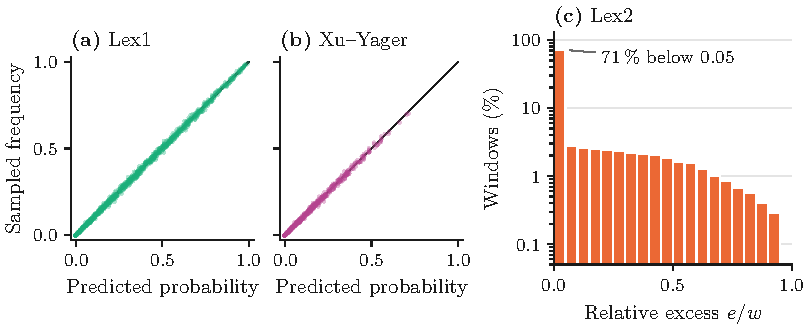
\includegraphics{Figure_4}
\caption{Simulation of single $2\times2$ windows with independent random intervals ($20000$ windows, $2000$ samples each). (a), (b) Violation probability of a window predicted by \Cref{prop:violation} against the frequency observed in the samples, for Lex1 and Xu--Yager ($3000$ windows shown each); points on the diagonal agree. (c) Excess width of Lex2 relative to the width of its output (\Cref{prop:excess}), on a logarithmic scale; the excess is zero in $68\%$ of the windows.}
\label{fig:sim}
\end{figure}

\paragraph{H3 (Lex2 is wider)} Confirmed. On the same lattice-trained weights, the logit interval of Lex2 is on average $0.9\%$ and $5.8\%$ wider than that of the lattice maximum on CIFAR-10 ($2/255$, $8/255$), $3.1\%$ and $14.7\%$ wider on MNIST ($0.1$, $0.3$), and $19.0\%$ wider on Fashion-MNIST (\Cref{fig:width}). Within each dataset the excess grows with the radius. For Lex2-trained weights it is $0.9\%$, $2.2\%$, $2.7\%$, $2.6\%$ and $9.5\%$: smaller in every case except CIFAR-10 $2/255$, where it is unchanged. Lex1 gives intervals $0.1\%$ to $1.5\%$ \emph{narrower} than the lattice maximum on every benchmark. Since the lattice maximum is the smallest enclosing selection (\Cref{prop:lattice}), this narrowing is width that Lex1 gains by dropping part of the range. Xu--Yager stays within $0.4\%$ of the lattice width in both directions.

With two pooling layers the excess of Lex2 compounds, as \Cref{thm:compare} allows. On lattice-trained weights its logit interval is $2.3\%$ and $12.7\%$ wider on CIFAR-10 ($2/255$, $8/255$) and $10.0\%$ and $75.4\%$ wider on MNIST ($0.1$, $0.3$). That is $2.2$ to $5.1$ times the excess with one pooling layer. The smallest ratio in any single network is $1.017$, so the inclusion of \Cref{thm:compare} holds for two pooling layers. At MNIST $0.3$ the ratio varies between $1.54$ and $1.88$ over the seeds. For Lex2-trained weights the excess is $1.8\%$, $5.6\%$, $10.4\%$ and $9.6\%$, again smaller except at MNIST $0.1$, where it is essentially unchanged. Lex1 is $0.7\%$ to $2.7\%$ narrower than the lattice maximum, and Xu--Yager stays within $0.3\%$ of it.

\begin{figure}[!ht]
\centering
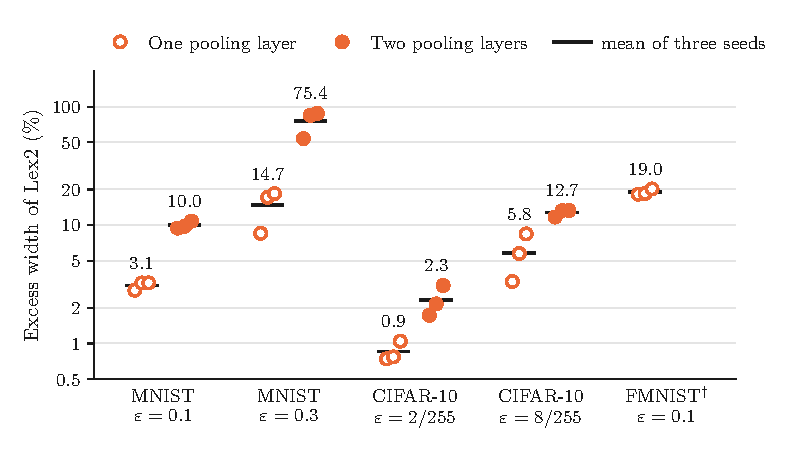
\includegraphics{Figure_5}
\caption{Excess width of Lex2 over the lattice maximum on lattice-trained weights. Each marker is one network: the width of the predicted logit's interval with Lex2 relative to the lattice maximum on the same weights, minus one, on a logarithmic scale. Bars and numbers give the mean over three seeds. Every value is positive, as \Cref{thm:compare} requires. $^\dagger$Earlier training recipe (\Cref{sec:fmnist}).}
\label{fig:width}
\end{figure}

\paragraph{H4 (verified accuracy)} Confirmed on fixed weights. Swapping Lex2 into a lattice-trained network lowers verified accuracy by $0.16$ and $1.85$ points on MNIST ($0.1$, $0.3$), $0.11$ and $0.67$ points on CIFAR-10 ($2/255$, $8/255$) and $1.42$ points on Fashion-MNIST. Training with Lex2 behaves differently on the two datasets. Compare the Lex2-trained network, evaluated with Lex2, against the lattice-trained network evaluated with the lattice maximum. On MNIST and Fashion-MNIST the gap shrinks to $-0.01$, $0.46$ and $0.16$ points: training recovers most of what the swap costs. On CIFAR-10 it grows to $0.49$ and $0.86$ points, larger than the swap cost, and is accompanied by the clean-accuracy loss at $8/255$. There the cost of Lex2 lies in the weights it produces, not only in its bounds. Evaluating Lex2-trained weights with the lattice maximum confirms this. On MNIST and Fashion-MNIST it gives the highest verified accuracy of all ($96.66\%$, $93.07\%$, $77.49\%$), but on CIFAR-10 it stays below the lattice-trained networks ($52.75\%$ against $53.08\%$, $33.49\%$ against $34.11\%$).

With two pooling layers the swap costs $0.42$ and $11.87$ points on MNIST ($0.1$, $0.3$) and $0.33$ and $1.43$ points on CIFAR-10 ($2/255$, $8/255$). The $11.87$ points at MNIST $0.3$ match the $75\%$ excess width found under H3. Training with Lex2 again behaves differently on the two datasets. On MNIST the trained gap is smaller than the swap cost, $0.11$ and $2.33$ points: training recovers four fifths of the loss at $\eps=0.3$ but not all of it. On CIFAR-10 it is larger, $0.66$ and $2.34$ points. Evaluating Lex2-trained weights with the lattice maximum gives the best verified accuracy only at MNIST $0.1$ ($96.97\%$ against $96.74\%$). At MNIST $0.3$ and on CIFAR-10 it stays below the lattice-trained network ($90.45\%$ against $91.66\%$, $52.35\%$ against $52.76\%$, $31.50\%$ against $33.33\%$).

\section{Discussion}
\label{sec:discussion}

\paragraph{Theory and experiment agree on fixed weights} The four operators behave as \Cref{thm:char,thm:compare} predict on every benchmark, with one and with two pooling layers. Lattice and Lex2 enclose, Lex1 and Xu--Yager do not, and Lex2 is never tighter than the lattice maximum. The price of Lex2 grows with the radius: with one pooling layer its logit intervals are $0.9\%$ wider at CIFAR-10 $2/255$ and $14.7\%$ wider at MNIST $0.3$. This fits \Cref{prop:excess}, whose excess grows with the overlap of the intervals in a window, and larger radii produce more overlap. The price also grows with the number of pooling layers: with two, the same excess is $2.3\%$ and $75.4\%$. A plausible reason is that a second Lex2 layer receives inputs that the first has already widened, so its own excess comes on top of an excess carried from below. The total then grows faster than the number of layers.

\paragraph{What training adds} The theory compares operators on fixed weights and says nothing about the networks that training produces with each. Here the datasets disagree. On MNIST, a network trained with Lex2 adapts: its excess width falls to $2.6\%$ at $\eps=0.3$, it loses less than half a point to the lattice network, and its weights certify slightly better under the lattice maximum than the lattice-trained weights. On CIFAR-10 the excess width also falls at $8/255$ (from $5.8\%$ to $2.2\%$), but the Lex2 network certifies fewer inputs and, at $8/255$, classifies fewer clean inputs correctly. A plausible explanation is the gradient routing of \Cref{prop:grad}. Under Lex2 the gradient of both endpoints reaches only the window element with the largest upper bound. On MNIST, where windows are usually dominated by one element anyway, this costs little. On CIFAR-10, with richer features and more overlap, it withholds signal from the element with the largest lower bound. We have not tested this explanation. With two pooling layers the same split between the datasets appears, but the cost of training with Lex2 is larger everywhere except at MNIST $0.1$. It reaches $2.3$ points of verified accuracy at MNIST $0.3$ and CIFAR-10 $8/255$, where three seeds now suffice to separate it from $0$.

\paragraph{Soundness has to be tested where it can fail} Unsound pooling violated enclosure in a fraction of a percent of windows, by amounts comparable to the activations themselves. Yet on MNIST and CIFAR-10 with one pooling layer, sampling the logits did not reveal a single violation, and with two it revealed violations in only $8$ of $48$ unsound evaluations, at rates below $0.5\%$. The later layers and the margin of most inputs hide most of what happens at a pooling layer. Soundness of a pooling operator should therefore be established by proof, as in \Cref{thm:char}, or tested at the layer itself, never inferred from sampling the network output.

\paragraph{Limitations} We used one architecture family with at most two pooling layers, so \Cref{thm:compare} was tested for one and two pooling layers but not beyond. The pool2 network has about a quarter of the parameters of pool1, so the comparison between the two layouts mixes the effect of the second pooling layer with that of model size; only comparisons between operators within one layout are controlled. The window violation test covers only the first pooling layer. All models were trained with IBP; methods that mix IBP with tighter relaxations or adversarial training \cite{zhang2020crownibp,muller2023sabr,depalma2024} may weigh the excess width differently. Three seeds are enough to show the sign of most differences between operators but not to make them significant. Our reference reproduces \citet{shi2021} at two of four settings and is up to $1.4$ points below at the others. The violation rates come from sampling and are therefore lower bounds.

\section{Conclusion}
\label{sec:conclusion}

An admissible maximum of intervals encloses the range of the maximum if and only if the order is Lex2, and an admissible minimum if and only if it is Lex1; no admissible order is sound for both. Lex2 is never tighter than the lattice maximum, by an amount given in closed form, and it is neither inclusion-isotone nor continuous, yet networks built from it are sound. The experiments on MNIST and CIFAR-10 confirm these predictions on trained networks with one and two pooling layers. The unsound orders Lex1 and Xu--Yager violated enclosure in up to $1\%$ of pooling windows, almost always without a visible violation at the logits. Replacing the lattice maximum by Lex2 cost between $0$ and $0.9$ points of verified accuracy with one pooling layer and between $0.1$ and $2.3$ points with two. The excess width of Lex2 grew by a factor of $2$ to $5$ with the second layer. A single pooling layer cost nothing compared with a strided convolution.

For practice this gives a simple rule. In networks whose intervals must enclose, pooling should use the lattice maximum, which is sound, the tightest enclosing choice, and computed by two ordinary max-pooling calls. If an order-based selection is needed, for instance to return an input interval unchanged, Lex2 is the only admissible order that keeps the guarantee. The more pooling layers a network has, the stronger this rule becomes. The open questions are whether the CIFAR-10 cost of training with Lex2 comes from its gradient routing, how the excess compounds beyond two pooling layers, and whether the characterization extends to the rank-based and aggregation-based poolings of \Cref{sec:agg} in trained networks.

\appendix
% tables and figures of the appendix are numbered A.1, A.2, ...; \thesection already prints ``Appendix A''
\setcounter{table}{0}
\setcounter{figure}{0}
\crefalias{section}{appendix}

\section{Fashion-MNIST with the earlier recipe}
\label{sec:fmnist}

Before switching to the recipe of \Cref{sec:method}, we trained the pooled CNN-7 on Fashion-MNIST \cite{xiao2017fmnist} at $\eps=0.1$. That recipe mixed the clean and robust losses ($\kappa$ from $1$ to $0.5$), used logit intervals instead of margin bounds and a linear $\eps$ ramp of $40$ epochs, had no warm-up regularizers, trained for $100$ epochs on $90\%$ of the training split, and kept the epoch with the best validation verified accuracy. These numbers can therefore not be compared with \Cref{tab:train} or with published results, only with each other (\Cref{tab:fmnist}).

\begin{table}[ht]
\centering\small
\setlength{\tabcolsep}{4pt}
\caption{Fashion-MNIST, earlier recipe, trained at $\eps=0.1$: clean and verified test accuracy (\%), mean $\pm$ standard deviation over three seeds. Bold: best among the IBP-trained models.}
\label{tab:fmnist}
\begin{tabular}{lcccc}
\toprule
Model & Clean & \multicolumn{3}{c}{Verified at $\eps$} \\
\cmidrule(lr){3-5}
 & & $0.025$ & $0.05$ & $0.1$ \\
\midrule
CNN-7, no pooling$^{\mathrm{a}}$ & $\mathbf{87.6}$ & $85.3$ & $82.8$ & $76.5$ \\
Pooled, lattice  & $87.43\pm0.13$ & $85.37\pm0.05$ & $83.00\pm0.17$ & $\mathbf{77.00\pm0.15}$ \\
Pooled, Lex2     & $87.38\pm0.14$ & $\mathbf{85.43\pm0.09}$ & $\mathbf{83.06\pm0.08}$ & $76.84\pm0.07$ \\
Pooled, standard & $94.15\pm0.20$ & $0.00$ & $0.00$ & $0.00$ \\
\bottomrule
\end{tabular}
\par\smallskip
\parbox{\linewidth}{\footnotesize $^{\mathrm{a}}$One seed.}
\end{table}

As on MNIST at $\eps=0.1$, the two sound operators are close. At the training radius, lattice minus Lex2 is $0.15\pm0.31$ points verified and $0.05\pm0.51$ points clean, paired by seed; at the smaller radii Lex2 is ahead by $0.06$ points, also within the seed-to-seed variation. \Cref{tab:main-fmnist} evaluates these networks with every pooling operator on the same weights, as \Cref{tab:main} does for the main benchmarks.

% generated by notebooks/A_analysis.ipynb; do not edit by hand
\begin{table}[tbp]
\centering\footnotesize
\setlength{\tabcolsep}{3.5pt}
\caption{Fashion-MNIST networks of the earlier recipe (one pooling layer) evaluated with every pooling operator on the same weights.}
\label{tab:main-fmnist}
\begin{tabular}{llccccc}
\toprule
Weights & Pooling & Window viol. & Max excess & Logit viol. & Verified & Width ratio \\
\midrule
\multicolumn{7}{l}{\emph{Fashion-MNIST $0.1$}} \\
\addlinespace[2pt]
Lattice & Lattice & $0$ & $1.6\cdot10^{-5}$ & $0$ & $77.00\pm0.15$ & $1.000$ \\
Lattice & Lex2 & $0$ & $1.6\cdot10^{-5}$ & $0$ & $75.58\pm0.11$ & $1.190$ \\
Lattice & Lex1 & $2.6\cdot10^{-3}$ & $2.0\cdot10^{0}$ & $4.4\cdot10^{-3}$ & n/a & $0.985$ \\
Lattice & Xu--Yager & $1.7\cdot10^{-3}$ & $4.3\cdot10^{-1}$ & $9.3\cdot10^{-4}$ & n/a & $0.996$ \\
Lex2 & Lex2 & $0$ & $6.6\cdot10^{-6}$ & $0$ & $76.84\pm0.07$ & $1.095$ \\
Lex2 & Lattice & $0$ & $5.2\cdot10^{-6}$ & $0$ & $\mathbf{77.49\pm0.05}$ & $1.000$ \\
\bottomrule
\end{tabular}
\par\smallskip
\parbox{\linewidth}{\footnotesize Window viol.\ and logit viol.: fractions of the windows of the first pooling layer and of the (input, logit) pairs whose sampled values leave the computed interval by more than $10^{-4}$ and $10^{-5}$. Max excess: largest distance of a sampled window maximum outside its interval, over seeds. Verified: verified accuracy in \%, mean $\pm$ standard deviation over three seeds, reported only for enclosing operators; bold marks the best per benchmark. Width ratio: mean width of the predicted logit relative to the lattice operator on the same weights. Clean accuracy does not depend on the operator and is given in \Cref{tab:fmnist}.}
\end{table}


\paragraph{Sanity checks on the earlier reference models} For each dataset, sampling $200$ points from the input box found no enclosure violation larger than $0$ (threshold $10^{-5}$), in agreement with \Cref{lem:layers}.

\section*{CRediT authorship contribution statement}
\textbf{Mohammadmahdi SharifBeygi:} Conceptualization, Methodology, Formal analysis, Software, Validation, Writing -- original draft, Writing -- review \& editing.
\textbf{Akbar Dehghan Nezhad:} Conceptualization, Methodology, Formal analysis, Supervision, Writing -- review \& editing.

\section*{Declaration of competing interest}
The authors declare that they have no known competing financial interests or personal relationships that could have appeared to influence the work reported in this paper.

\section*{Funding}
This research did not receive any specific grant from funding agencies in the public, commercial, or not-for-profit sectors.

\section*{Data availability}
All datasets analyzed during the current study (MNIST, Fashion-MNIST, and CIFAR-10) are publicly available benchmark datasets.

\section*{Code availability}
The source code for all pooling operators, certified-training pipelines, and experiments reported in this paper is publicly available at
\begin{center}
  \url{https://github.com/MohammadMahdi-Sharifbeigy/admissible-pooling}
\end{center}
The repository includes the \texttt{interval\_gnn} PyTorch library implementing the Lattice, Lex2, Lex1 and Xu--Yager pooling operators, all experiment configuration files (Drafts~A), training and evaluation scripts, and the Jupyter notebooks used to produce the figures in this paper.

\bibliographystyle{elsarticle-num-names}
\bibliography{refs}

\end{document}
